\documentclass[a4paper]{scrreprt}
\usepackage[german]{babel}
\usepackage[utf8]{inputenc}
\usepackage{graphicx}
\usepackage{pdflscape}

\begin{document}
\chapter{Implementierungsplanung}
Die Packages (hier fett) sind mit allen ihren Meilensteinen jeweils einem der Phasenverantwortlichen zugeordnet. \\
Die Meilensteinen sind Personen zugeordnet. \\
Die Zahl in der Klammer jedes Meilensteins erklärt, in der wievielten Woche der Meilenstein implementiert werden soll. \\
\begin{tabular}{ | p{7cm} | p{7cm} |}
    \hline
	Was & Wer\\
	\hline
	
	\rule{0pt}{15pt}\textbf {CodeArea} & Schnell\\
	&\\
	\hline
	Interfaces (1) & Klein\\
	\hline
	Basisimplementierung (1-2) & Schnell und Klein\\
	\hline
	Syntaxhighliting (3) & Schnell \\
	\hline
	Kannkriterien (4) & Schnell und Klein \\
	\hline
	
	\rule{0pt}{15pt}\textbf {CElectionDescriptionEditor} & Schnell\\
	&\\
	\hline
	GUI-Dummy (1) & Klein \\
	\hline
	GUI-Funktionalität (2) & Klein\\
	\hline
	Interfaces (1) & Klein\\
	\hline
	Speichern und Laden (3) & Klein\\
	\hline
	Fehlererkennung (2-3)& Klein\\
	\hline
	Kannkriterien (4) & Klein\\
	\hline
	
	\rule{0pt}{15pt}\textbf {BooleanExpEditor} &  Schnell \\
	&\\
	\hline
	Interfaces (1) & Schnell\\
	\hline
	GUI-Dummy (1) & Schnell\\
	\hline
	GUI-Funktionalität (2) & Schnell\\
	\hline
	Speichern und Laden (3) & Schnell\\
	\hline	
	Fehlererkennungskommunikation (2) & Schnell\\
	\hline
	Kannkriterien (4) & Schnell\\
	\hline
	
	\rule{0pt}{15pt}\textbf {PropertyList} & Hanselmann\\
	&\\
	\hline
	Interfaces (1) & Hecht\\
	\hline
	GUI-Dummy (1) & Hecht\\
	\hline
	GUI-Funktionalität (2)& Hecht\\
	\hline
	Speichern und Laden (3)& Hecht\\
	\hline
	Ergebnisdarstellung (2-3) & Hecht\\
	\hline	
	
	\rule{0pt}{15pt}\textbf {Options} & Hanselmann\\
	&\\
	\hline
	Interfaces (1) & Stapelbroek\\
	\hline
	Basisimplementierung (1-2) & Stapelbroek\\
	\hline
	Kannkriterien (4) & Wohnig \\
	\hline
	
\end{tabular}\\
\\
\begin{tabular}{ | p{7cm} | p{7cm} |}
	\hline
	Was & Wer\\
	\hline
	
	\rule{0pt}{15pt}\textbf {PropertyChecker} & Hanselmann\\
	&\\
	\hline
	Interfaces (1) & Hanselmann\\
	\hline
	CBMC-Ansteuerung (2-3) & Stapelbroek \\
	\hline
	Codegenerierung (2-3) & Hanselmann und Stapelbroek \\
	\hline
	Eventuelle Multithreadingverbesserung (4) & Stapelbroek \\
	\hline
	
	\rule{0pt}{15pt}\textbf {Parametereditor} & Hanselmann \\
	&\\
	\hline
	Interfaces (1) & Wohnig\\
	\hline
	GUI-Dummy (1) & Wohnig\\
	\hline
	GUI-Funktionalität (2) & Wohnig\\
	\hline
	Speichern und Laden (3) & Wohnig\\
	\hline
	
	\rule{0pt}{15pt}\textbf {DataTypes} & Hanselmann\\
	&\\
	\hline
	Implementierung (1) & Stapelbroek und Hanselmann\\
	\hline	
	
	\rule{0pt}{15pt}\textbf {Toolbox} & Schnell\\
	&\\
	\hline	
	ANTLRHandler (2-3)  & Schnell\\
	(Erstellung des AST, Fehlererkennung in den formalen Eigenschaften) &\\
	\hline
	UserActionKlasse (1-2) & Wohnig\\
	\hline
	
	\rule{0pt}{15pt}\textbf {StringRessource} & Hanselmann\\
	&\\
	\hline	
	Interface (1) & Hanselmann \\
	\hline
	Anlegen und verwalten der Textdatei Deutsch (1) & Hanselmann \\
	\hline
	Anlegen Textdatei Englisch (4) & Hanselmann \\
	\hline
	
	\rule{0pt}{15pt}\textbf {SaverLoader} & Hanselmann\\
	&\\
	\hline
	Interfaces (1) & Hecht\\
	\hline	
	
	\rule{0pt}{15pt}\textbf {HighLevel} & Hanselmann\\
	&\\
	\hline
	Komplette Implementierung (1) & Wohnig\\
	\hline
	
	\rule{0pt}{15pt}\textbf {Sonstiges} & Hanselmann\\
	&\\
	\hline
	Erstellung JAR (1) & Wohnig \\
	\hline
	Präsentationsplanung (4) & Schnell und Hanselmann  \\
	\hline
	Änderungsdokument erstellen (1-4) & Wohnig \\
	\hline
	
    \end{tabular}\\\\

Hier die Formatierung nach Personen sortiert: \\\\
Schnell:
\begin{itemize} 
\item BooleanExpEditor Interfaces (1)
\item BooleanExpEditor GUI-Dummy (1)
\item CodeArea Basisimplementierung [mit Klein] (1-2)
\item BooleanExpEditor GUI-Funktionalität (2)
\item BooleanExpEditor Fehlererkennungskommunikation (2) 
\item Toolbox ANTLRHandler [mit Schnell] (2-3) 
\item CodeArea Syntaxhighliting (3)
\item BooleanExpEditor Speichern und Laden (3) 
\item BooleanExpEditor Kannkriterien (4)
\item CodeArea Kannkriterien [mit Klein] (4)
\item Sonstiges Präsentationsplanung [mit Hanselmann] (4)
\end{itemize} 
\vspace{8mm}
Klein: 
\begin{itemize}
\item CodeArea Interfaces (1)
\item CElectionDescriptionEditor GUI-Dummy (1) 
\item CElectionDescriptionEditor Interfaces (1)
\item CodeArea Basisimplementierung [mit Schnell] (1-2)
\item CElectionDescriptionEditor GUI Funktionalität (2)
\item CElectionDescriptionEditor Fehlererkennung (2) 
\item Toolbox ANTLRHandler [mit Schnell] (2-3) 
\item CElectionDescriptionEditor Speichern und Laden (3)
\item CodeArea Kannkriterien [mit Schnell] (4)
\item CElectionDescriptionEditor Kannkriterien (4)
\end{itemize} 
\vspace{8mm}
Hecht: 
\begin{itemize}
\item PropertyList Interfaces (1)
\item PropertyList GUI-Dummy (1)
\item PropertyList GUI-Funktionalität (2)
\item PropertyList Ergebnisdarstellung (2-3)
\item PropertyList Speichern und Laden (3)
\item StringRessource Anlegen Textdatei Englisch (4)
\end{itemize} 
\vspace{8mm}
Stapelbroek:
\begin{itemize}
\item Datatypes Implementierung [mit Hanselmann] (1)
\item Options Interface (1)
\item Options Basisimplementierung Implementierung (1-2)
\item PropertyChecker CBMC-Ansteuerung (2-3) 
\item PropertyChecker Codegenerierung [mit Hanselmann] (2-3) 
\item PropertyChecker Eventuelle Multithreadverbesserung (4)
\end{itemize}
\vspace{8mm}
Hanselmann:
\begin{itemize}
\item Datatypes Implementierung [mit Stapelbroek] (1)
\item PropertyChecker Interfaces (1)
\item SaverLoader Interface (1)
\item StringRessource Interface (1)
\item StringRessource Anlegen und verwalten der Textdatei Deutsch (1)
\item PropertyChecker Codegenerierung [mit Stapelbroek] (2-3)
\item Sonstiges Präsentationsplanung [mit Schnell] (4)
\end{itemize}
\vspace{8mm}
Wohnig:
\begin{itemize}
\item Parametereditor Interfaces (1)
\item Parametereditor GUI-Dummy (1)
\item HighLevel Komplette Implementierung (1)
\item Sonstiges Erstellung JAR (1)
\item Toolbox UserActionKlasse (1-2)
\item Parametereditor GUI-Funktionalität (2)
\item Parametereditor Speichern und Laden (3)
\item Sonstiges Änderungsdokument erstellen (1-4)
\item Options Kannkriterien (4)
\end{itemize}
\vspace{8mm}
In dem folgenden Diagramm sieht man die Zeitplanung: \\
\begin{landscape}
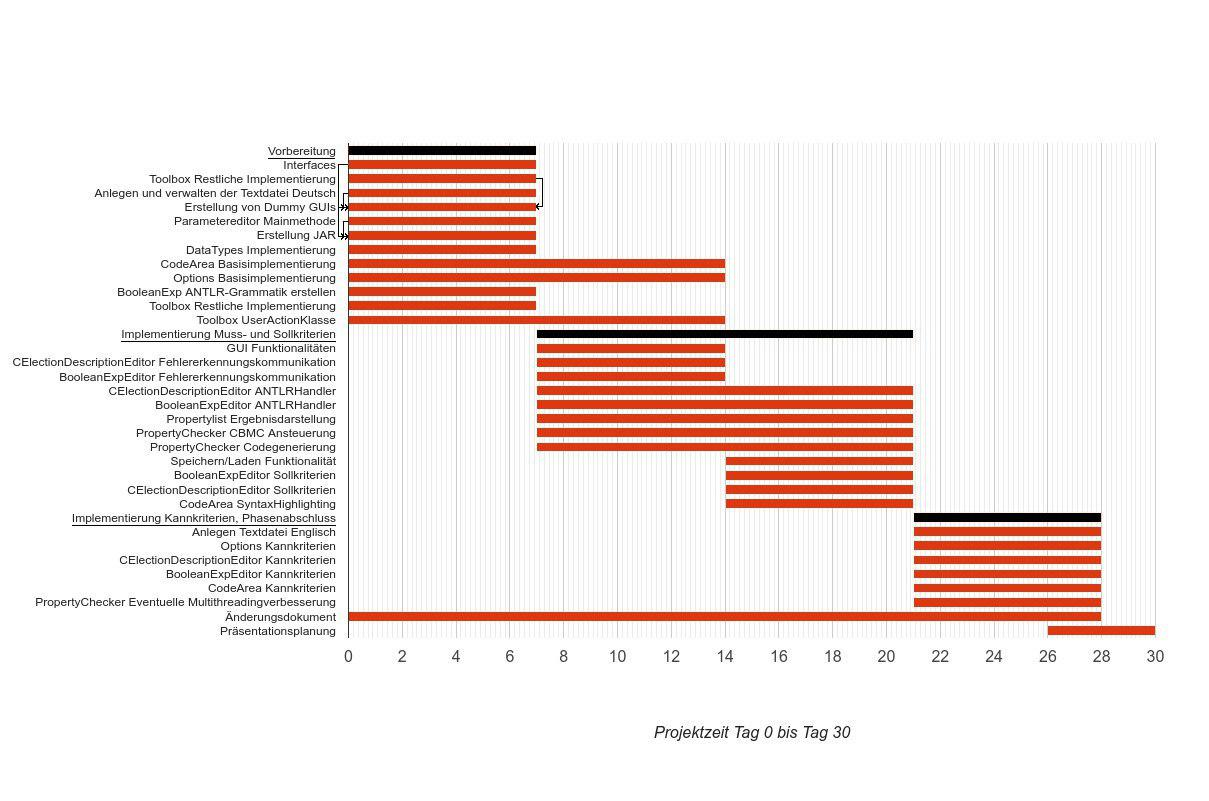
\includegraphics[width=1.4\textwidth] {planung.jpg}
\end{landscape}


\end{document}